\documentclass[../../main.tex]{subfiles}

\begin{document}

\chapter{Quadratics}

\section{What is a quadratic equation?}
% consider adding intro here - cyanine
A \b{quadratic equation} in terms of $x$ is any equation that can be written in the form 

{\hfill\Large\bfseries NEEDS FIXING\hfill}
\begin{lstlisting}
\begin{formula}
ax^2+bx+c=0
\end{formula}
 \end{lstlisting}
where $a,b,c$ are real constants, and $a\neq0$. We say "can be written in the form" because they aren't always given as such, sadly. Here are all examples of quadratic equations:
\begin{align}
    x^2+3x+1&=0 & 2x-1&=x^2 & x^2 + 1 &= 0 \\
    \frac{x^2}{2}-30x+19^{\frac74}&=0  & (x-15)^2&=0  & 5+4x^2&=3x \\
    (x-10^{-420})(x-\sqrt{3})&=0 & -24x&=x^2+144 & (-2)^3&=(x-1)^2
\end{align}
You should be able to convince yourself that, with some algebraic manipulation, all of these equations can be written in the form above.

\begin{insight}{Sneaky Quadratics}
Don't assume that quadratic equations are always in terms of $x$ either - sometimes you can have quadratics of other functions as well. Take one example: $$x+1=2\sqrt{x}$$ This doesn't look like a quadratic equation at first, but some quick work reveals $$(\sqrt{x})^2-2(\sqrt{x})+1=0$$ which is a quadratic in terms of $\sqrt{x}$! You can then solve this as a quadratic equation to get $\sqrt{x}=1$, which gives $x=1$. Be on the lookout for equations like this - note though, that solutions of the quadratic may lie outside the function's domain, and thus might be invalid.
\end{insight}

%%% note: have rshields check the last line - cy

A \b{solution} of a quadratic equation is any value of $x$ that makes the given equation true. For example, a solution for the middle equation is $x=15$.

Quadratic equations can have either \b{two, one, or zero real solutions}. Incidentally, the left column of equations above returns two solutions, the middle one, and the right none. How do we know this?
\newpage
There are a couple of ways of finding the solution(s) to a quadratic:
\begin{itemize}
    \item \b{Factorization}
    \item \b{Completing the square}
    \item Using \b{Vieta's formula}
    \item Using the \b{quadratic formula}
    \item \b{Graphing} (either by hand or using technology)
\end{itemize}

Hopefully you're good with factorizing trinomials in Chapter 1 - if not, go back and have a review. We'll be looking at the other methods one by one.

\section{Completing the Square}
When given a quadratic equation, the first thing you should do is collect all the terms to one side, and convert it into the familiar form $ax^2+bx+c=0$. Unless the equation is already simple enough, this makes it easier to handle. You may also want to divide the equation by $a$ if it divides both $b$ and $c$ - but to make things neater, here we've divided through regardless.

Let's assume we've done both of the above. We currently have a quadratic of the form $x^2+Bx+C=0$, where $B=\frac{b}{a}$ and $C=\frac{c}{a}$. It'd be even better if this were a linear equation - can we reduce it into one?

We can use the \b{square of sums/differences} formula to perform some manipulations:
\begin{align}
    x^2+Bx+C=0\therefore\ &x^2+Bx=-C \\
    \therefore\ &x^2+2\frac{B}2x+\left(\frac{B}{2}\right)^2=-C+\left(\frac{B}{2}\right)^2 \\
    \therefore\ &\left(x+\frac{B}{2}\right)^2=\frac{B^2}{4}-C \\
    \implies&x+\frac{B}{2}=\pm\sqrt{\frac{B^2}{4}-C}
\end{align}
Note the equation on the last line: the right side is now a constant, so we just need to move $\dfrac B2$ over and be done. \b{Remember the plus/minus symbol on the right side, by the way} - it signifies both of our solutions.

Should we see how this is applied?

\newpage\begin{example}{Completing the Square}
By completing the square, solve $2x^2-12x+1=0$.

\sep
We have:
\begin{align}
    2x^2-12x+1=0\implies& x^2-6x=-\frac12 \\
    \therefore\ & (x-3)^2\equiv x^2-6x+9=\frac{17}2 \\
    \therefore\ & x=3\pm\sqrt{\frac{17}{2}}.
\end{align}

\end{example}

\begin{thinking}{~}
Given our previous working with the (simplified) quadratic $x^2+Bx+C=0$, when do you think the quadratic equation would have two solutions? One? None? \b{Bonus:} Also... hmmm, doesn't the general form of the solution look familiar?
\end{thinking}
\begin{questions}{Drills}
By completing the square, solve the following quadratic equations for real $x$.
\begin{question_set}(2)
    \item $(x-4)^2=3x$
    \item $x-4=3x^2$
    \item $x^2+\dfrac{4x}{3}=-\dfrac{4}{9}$
    \item $x^2+1=(3x-4)^2$
    \item $10x=x^2-(2x+3)^2$
    \item $(x+1)^2=2x$
\end{question_set}
\end{questions}


\section{Vieta's Formula}
Again, here we assume that you are already familiar with the \b{factorization} of quadratics; if not, you can go back and review in Chapter 1.

Let's assume this time that \i{we already know our quadratic equation has at least one solution}. In this case, our quadratic can also be written in the factorized form
\begin{equation*}
    ax^2+bx+c=0\implies a(x - \beta)(x - \gamma) = 0
\end{equation*}
where $\beta,\gamma$ are the solution of our equation. In this case, how would we find $\beta$ and $\gamma$ in terms of our coefficients $a, b$, and $c$?

Expanding gives us:
\begin{align}
    a(x-\beta)(x-\gamma)
    &= ax^2-a(\beta+\gamma)x+a\beta\gamma \\
    &\equiv ax^2+bx+c.
\end{align}
By comparing the last two expressions, we see that
$$-a(\beta+\gamma)=b\qquad\rm{and}\qquad a\beta\gamma=c\rm{, or}$$
$$\beta+\gamma=-\frac{b}{a},\qquad\beta\gamma=\frac{c}{a}.$$
This relationship has a special name - \b{Vieta's formula}! To summarize:
\begin{theorem}{Vieta's Formula}
If a quadratic equation has form $ax^2+bx+c=0$, then its solutions are given by $$r_1+r_2=-\frac{b}{a}\qquad\rm{and}\qquad r_1r_2=\frac{c}{a}.$$
\end{theorem}

Why is this useful? %%% add short blurb here - cy

\begin{example}{Applying Vieta's Formula}
Solve for $x$: $$2x^2-8x-42=0$$

\sep
We have:
$$\begin{cases}
        r_1+r_2=4 \\
        r_1r_2=-21
    \end{cases}$$
A quick inspection shows that the pair of values $r_1=7$ and $r_2=-3$ is the solution to this equation.
\end{example}
Note that, in the context of quadratic equations, \i{Vieta's formula is more often used as a calculation shortcut for neat cases than as a fits-all method.} That said, it \i{is} especially useful when said cases do occur.
\begin{insight}{~}
"Oh, \i{another} formula to remember", you'd say, but it so happens that questions like this come up quite often. They're so frequent because they're designed to make things quick, and allow you to spend more time on the later questions. Try to think of it as a hack, a time-saving cheat, instead of just as a menial piece of trivia.
\end{insight}

\begin{questions}{Drills}
Can these quadratic equations be quickly solved with Vieta's formula? If so, simplify the equation and write down the solution(s). Otherwise, try completing the square and solve.
\begin{question_set}(2)
    \item $x^2-6x-91=0$
    \item $ $
    \item $ $
    \item $ $
    \item $ $
    \item $ $
\end{question_set}
\end{questions}

\section{The Quadratic Formula}
Now we have the final analytical method given, which is the \b{quadratic formula}. Many of you might already be familiar with this; regardless, it is given below:

{\hfill\Large\bfseries NEEDS FIXING\hfill}
\begin{lstlisting}
\begin{formula}
ax^2+bx+c=0 $$$$
\implies x=\frac{-b\pm\sqrt{\Delta}}{2a},\ \Delta=b^2-4ac
\end{formula}
 \end{lstlisting}
where $\Delta$ is called the \b{discriminant} of the equation. The proof, though probably not as commonly given, is actually not too complex. As motivation, we'll leave it as an exercise.

The special value $\Delta=b^2-4ac$ is called the discriminant because it allows us to deduce certain things about the quadratic equation. At the start of the chapter, we asked how we would identify whether a quadratic would have two, one, or zero solutions. The discriminant tells us exactly that:

\begin{theorem}{Discriminant and Number of Solutions}
For any quadratic equation $ax^2+bx+c=0$, if $\Delta=b^2-4ac$,
$$\begin{cases}
    \Delta>0\implies\rm{two real solutions,} \\
    \Delta=0\implies\rm{one real solution,} \\
    \Delta<0\implies\rm{no real solutions.}
\end{cases}$$
\end{theorem}
\begin{thinking}{~}
Why is the above theorem true?
\end{thinking}
Some questions might ask you to find the values for each constant that satisfy one or more of the above three cases. The discriminant then becomes a useful tool in evaluating the quadratic's behavior. Here's an example.
\begin{example}{To Have a Solution}
Find all real values of $m$ such that $$(m-2)x^2-2x-4=0$$ has at least one solution.
\sep
Be careful - having at least one solution means that we can either have one or two of them. We can infer that $\Delta\geq0$, and we have
\begin{align}
    \Delta&\equiv(-2)^2-4(m-2)(-4)\geq0 \\
    &\therefore16m-28\geq0 \\
    &\therefore m\geq\frac74.
\end{align}
\end{example}

\subsection{Special Cases of Quadratic Equations}
Before we conclude the analytical (written) methods section, let's have a look at some special cases. The above formulae are certainly very useful, but it's not like we have to mechanically apply them every single time, right?
\begin{example}{Simple Enough}
Solve for real $x$:
\begin{question_set}(2)
    \item $x^2=4x$
    \item $(x-4)^2=(2x+3)^2$
\end{question_set}
\sep
1. It's uncommon, but possible, to miss a solution by dividing the equation through by $x$. This assumes that $x\neq0$; however, $x=0$ is indeed a solution of this equation. A quick factorization gives $$(1)\implies x^2-4x=0\therefore x(x-4)=0\therefore x=0\rm{ or } x=4.$$
To be fair, you could've also just eyeballed the solutions.

2. Taking \i{both the positive and negative} square roots on both sides gives two cases:
\begin{align}
    &\begin{cases}x-4=2x+3\\x-4=-2x-3\end{cases} \\
    \therefore&\begin{cases}x=-7\\x=\frac13.\end{cases}
\end{align}
\end{example}
In general, try to be flexible in your working whenever possible. Make sure you have a proper understanding of how each method's used, and practice until you're comfortable with adapting to various question types. Revise when necessary, of course - juggling between methods can be challenging!

%%% might wanna revise this later - cy

There's no drills for this subsection - check the exercises at the end, and apply shortcuts like these whenever suitable.

\section{Graph of a Quadratic Function}
The last method we'll be going over is a visual one. It helps if you're a visual thinker, but know that you'll have to be able to identify graphs of quadratic equations, as well as their characteristics when asked.

By considering the left side of the quadratic equation $ax^2+bx+c=0$ as $f(x)=0$, we can reframe our question as finding the $x$-intercepts of the function $y=f(x)$ (if they exist, of course). The $x$-coordinate of such intercepts - the $x$-values where $f(x)=0$ - are called the \b{roots} of our function. 
\begin{insight}{Roots vs. Solutions}
Roots are a characteristic of a function; they're not the same as solutions, which are characteristics of an equation. If $x_1, x_2$ are the \i{roots} of some \i{function} $f(x)$, then they are also (well, by definition) the \i{solutions} to the \i{equation} $f(x)=0$. It might be helpful to keep that small distinction in mind.
\end{insight}

If all you're trying to do is finding the roots, this might be overkill - but that's what GDCs are for, right?

It takes a quadratic function to know one, so here are a few examples:
\begin{center}
    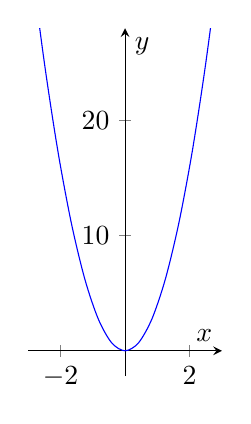
\begin{tikzpicture}
        \begin{axis}
        [height=6cm,width=\textwidth/3,
        axis y line = center,
        axis x line = middle,
        xlabel=$x$,ylabel=$y$,
        xmin=-3,xmax=3, ymin=-2.2,ymax=28]
            \addplot[smooth, blue, mark = none]{4*x^2};
        \end{axis}
    \end{tikzpicture}\qquad\qquad
    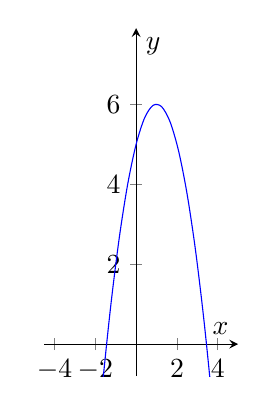
\begin{tikzpicture}
        \begin{axis}
        [height=6cm,width=\textwidth/3,
        axis y line = center,
        axis x line = middle,
        xlabel=$x$,ylabel=$y$,
        xmin=-4.5,xmax=5, ymin=-0.8,ymax=7.9]
            \addplot[smooth, blue, mark = none]{-x^2 + 2*x + 5};
        \end{axis}
    \end{tikzpicture}\qquad\qquad
    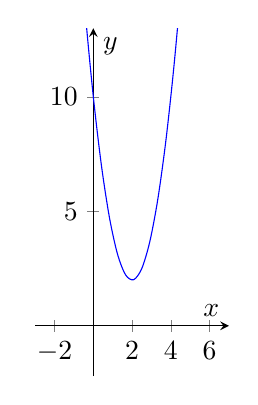
\begin{tikzpicture}
        \begin{axis}
        [height=6cm,width=\textwidth/3,
        axis y line = center,
        axis x line = middle,
        xlabel=$x$,ylabel=$y$,
        xmin=-3,xmax=7, ymin=-2.2,ymax=13]
            \addplot[smooth, blue, mark = none]{2*x^2-8*x+10};
        \end{axis}
    \end{tikzpicture}
\end{center}

We can note that these quadratic functions take the shape of symmetric U-shaped curves (\b{parabolas}) that open either upwards or downwards. The values of $a, b, c$ determine the shape of the parabola, as well as the function's 

\end{document}